\documentclass[10pt,spanish]{article}  
\usepackage[spanish]{babel} %Indica que escribiermos en español
\usepackage[utf8]{inputenc} %Indica qué codificación se está usando ISO-8859-1(latin1)  o utf8 
\selectlanguage{spanish}

%%%%%%% DEFINICIÓN DE VARIABLES %%%%%%%%%%%%%%%%%%%
\newcommand{\Tarea}{Tarea \{ \# \}}
\newcommand{\Titulo}{Modelo de Dominio}
\newcommand{\Materia}{\{ MATERIA \}}
\newcommand{\Curso}{Curso \{ AÑO \}}
\newcommand{\Grupo}{Grupo \{ NRO \}}
% Nombre y Cedulas de los integrantes del grupo
\newcommand{\NomIntegrUno}{Integrante 1}
\newcommand{\CiIntegrUno}{CI}
\newcommand{\NomIntegrDos}{Integrante 2}
\newcommand{\CiIntegrDos}{CI}
\newcommand{\NomIntegrTres}{Integrante 3}
\newcommand{\CiIntegrTres}{CI}
\newcommand{\NomIntegrCuatro}{Integrante 4}
\newcommand{\CiIntegrCuatro}{CI}
\newcommand{\NomIntegrCinco}{Integrante 5}
\newcommand{\CiIntegrCinco}{CI}
% Nombre del Docente
\newcommand{\NomDocente}{Nombre Docente}
% Texto del Encabezado
\newcommand{\EncabezadoIzq}{Universidad de la República}
\newcommand{\EncabezadoMed}{Facultad de Ingeniería}
\newcommand{\EncabezadoDer}{Instituto de Computación}

%%%%%%%% PREÁMBULO %%%%%%%%%%%%

\usepackage{amsmath} % Comandos extras para matemáticas (cajas para ecuaciones,
% etc)
\usepackage{amssymb} % Simbolos matematicos (por lo tanto)
\usepackage{graphicx} % Incluir imágenes en LaTeX
\usepackage{color} % Para colorear texto
\usepackage{subfigure} % subfiguras
\usepackage{float} %Podemos usar el especificador [H] en las figuras para que se queden donde queramos
\usepackage{capt-of} % Permite usar etiquetas fuera de elementos flotantes
% (etiquetas de figuras)
\usepackage{sidecap} % Para poner el texto de las imágenes al lado
	\sidecaptionvpos{figure}{c} % Para que el texto se alinie al centro vertical
\usepackage{caption} % Para poder quitar numeracion de figuras
\usepackage{commath} % funcionalidades extras para diferenciales, integrales,
% etc (\od, \dif, etc)
\usepackage{cancel} % para cancelar expresiones (\cancelto{0}{x})


% MARGENES 
\usepackage{anysize} 					% Para personalizar el ancho de  los márgenes
\marginsize{2cm}{2cm}{2cm}{2cm} % Izquierda, derecha, arriba, abajo
\setlength{\parindent}{0cm}
\setlength{\parskip}{\baselineskip}

% Para que las referencias sean hipervínculos a las figuras o ecuaciones aparezcan en color
\usepackage[colorlinks=true,plainpages=true,citecolor=blue,linkcolor=blue]{hyperref}
%\usepackage{hyperref} 

% ENCABEZADO Y PIE DE PÁGINA
\usepackage{fancyhdr} 
\pagestyle{fancy}
\fancyhf{}

\fancyhead[L]{\EncabezadoIzq} %encabezado izquierda
\fancyhead[C]{\EncabezadoMed} %encabezado centro
\fancyhead[R]{\EncabezadoDer}   % dereecha

\fancyfoot[R]{\Curso}  % Pie derecha
\fancyfoot[C]{\thepage}  % centro
\fancyfoot[L]{\Tarea}  %izquierda
\renewcommand{\footrulewidth}{0.4pt}

\usepackage[framemethod=tikz]{mdframed}
\newmdenv[
  topline=false, %oculta linea arriba
  bottomline=false, % oculta linea abajo
  rightline=false, % oculta linea derecha
  skipabove=\topsep,
  skipbelow=\topsep,
]{siderules}

\numberwithin{figure}{section} % numeración de figuras por seccion
\usepackage[font=bf,labelfont=bf]{caption} % setea estilo bf (bold) a los caption (texto y label)

\usepackage[compact]{titlesec} %Formato de las secciones
\titleformat*{\section}{\LARGE\bfseries}
\titleformat*{\subsection}{\Large\bfseries}


\usepackage{etoolbox} % Agrega puntos a las sections en el TOC
\makeatletter
\patchcmd{\l@section}
  {\hfil}
  {\leaders\hbox{\normalfont$\m@th\mkern \@dotsep mu\hbox{.}\mkern \@dotsep mu$}\hfill}
  {}{}
\makeatother

\title{\Tarea - \Titulo}

%%%%%%%% TERMINA PREÁMBULO %%%%%%%%%%%%

\begin{document}

%%%%%%%%%%%%%%%%%%%%%%%%%%%%%%%%%% PORTADA %%%%%%%%%%%%%%%%%%%%%%%%%%%%%%%%%%%%%%%%%%%%
\begin{minipage}{0.48\textwidth} \begin{flushleft}
\end{flushleft}\end{minipage}

%%%
\begin{center}																		%%%
\newcommand{\HRule}{\rule{\linewidth}{0.5mm}}									%%%\left
 																					%%%


													 								%%%
\vspace*{1cm}								%%%
																				%%%	
\textsc{\huge \Materia}\\[1.5cm]	

\textsc{\huge \Tarea				%%%
}\\[1.5cm]													%%%

    																				%%%
\vspace*{1cm}																		%%%
																					%%%
\HRule \\[0.4cm]																	%%%
{ \huge \bfseries \Titulo}\\[0.3cm]	%%%
 																					%%%
\HRule \\[4cm]																	%%%
 																				%%%
																					%%%
\begin{minipage}{0.8\textwidth}													%%%
\begin{flushleft} \large															%%%
\textsc{\LARGE \Grupo}\\
\LARGE{\textbf{Integrantes}}\\	
\Large
\vspace{0.3cm}
  \begin{tabular}{ | p{10cm} | p{2.5cm} | }
    \hline
    \textbf{Nombre} & \textbf{CI} \\ \hline
    \NomIntegrUno & \CiIntegrUno \\ \hline
    \NomIntegrDos & \CiIntegrDos  \\ \hline 
    \NomIntegrTres & \CiIntegrTres \\ \hline
    \NomIntegrCuatro & \CiIntegrCuatro \\ \hline
    \NomIntegrCinco & \CiIntegrCinco \\ \hline
  \end{tabular}\\[0.5cm]
\LARGE{\textbf{Docente}}\\	
\Large
\vspace{0.3cm}
\begin{tabular}{ | p{10cm} |}
    \hline
     \NomDocente \\ 
     \hline
  \end{tabular}
\end{flushleft}																		%%%
\end{minipage}		
																%%%
\begin{minipage}{0.52\textwidth}		
\vspace{-0.6cm}											%%%
\begin{flushright} \large															%%%
\emph{} \\																	%%%
													%%%
\end{flushright}																	%%%
\end{minipage}	
\begin{flushleft}
 	
\end{flushleft}
%%%
 		\flushleft{\textbf{}	}\\																		%%%								  						
\end{center}							 											
																					
%%%%%%%%%%%%%%%%%%%% TERMINA PORTADA %%%%%%%%%%%%%%%%%%%%%%%%%%%%%%%%
\newpage
\tableofcontents

\newpage
\section{Introducción}
\subsection{Propósito}
El propósito de este documento es brindar una descripción general del Modelo de Dominio.

\subsection{Alcance}
El informe del Modelo de Dominio ilustra los conceptos del dominio identificados y sus relaciones, además de las restricciones de integridad que aplican sobre ellos. Incluye, además, información (parcial) acerca de los conceptos, los tipos de datos y las relaciones (principalmente las asociaciones) propiamente. 

\subsection{Estructura del Documento}
El documento está dividido en cuatro secciones. La segunda sección presenta el modelo conceptual con los conceptos del dominio y relaciones identificados. Por último, la tercera sección presenta las restricciones de integridad que aplican sobre los conceptos y relaciones identificados.

\begin{siderules}
A lo largo de esta plantilla se encuentran comentarios y ejemplos acerca del contenido del documento a elaborar a partir de ésta. Éstos se encuentran indicados, al igual que este párrafo, por una línea a lo largo de su borde izquierdo. Estas secciones deben ser eliminadas de la versión final del documento.
\end{siderules}

\section{Dominio del Problema}
Se presentan los principales conceptos del dominio del problema que se está modelando así como la relación que existe entre ellos. Se incluye un diagrama de clases expresando gráficamente estos conceptos y relaciones.

\begin{siderules}
A modo de ejemplo en la Figura 2.1 se muestra un modelo conceptual.\\
\begin{figure}[H] % Workaround para evitar error de floats: http://tex.stackexchange.com/a/290072/21357
    \centering    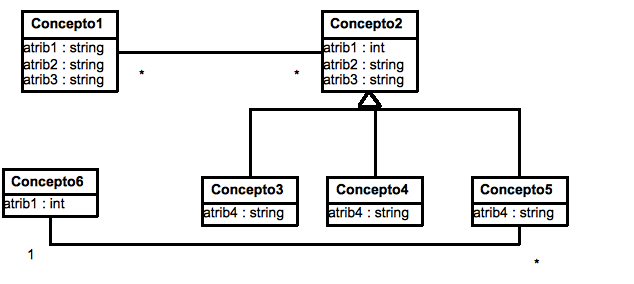
\includegraphics[]{ModeloDominio/Fig2-1.png}
    \caption{Modelo Conceptual del Sistema}
\end{figure}
\end{siderules}

\section{Restricciones}
En esta sección se presentan las restricciones que aplican al modelo. Estas restricciones refieren a los
elementos ilustrados en el diagrama de la sección anterior y están expresados en lenguaje natural.
\begin{siderules}
\begin{verbatim}
-- Restricción en lenguaje natural
-- ej: El valor de Atrib1 debe ser único para cada Concepto2
\end{verbatim}
\end{siderules}

\end{document}